Submitted:


\begin{minted}{text}
[1, 3]
\end{minted}


Chosen option 1 is available?\begin{quote}Yes.\end{quote}Chosen option 3 is available?\begin{quote}Yes.\end{quote}Remarks on your solution:

All given class diagrams are correct?

\begin{quote}
\begin{minted}{text}
No.
\end{minted}
\end{quote}

The correct solution is:
\begin{minted}{text}
[1,4]
\end{minted}


Your answer to class diagram 3 is not correct.

Class diagram 3 is invalid.

The relationships in the class diagram could be named in the following way:



\begin{centering}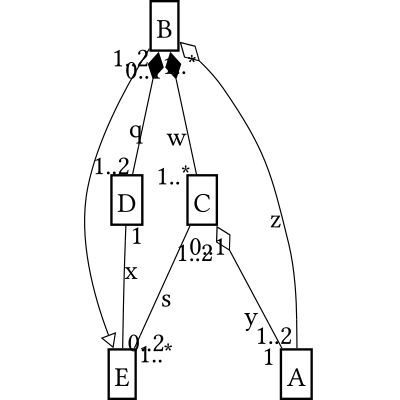
\includegraphics[min width=0.4\textwidth=0.6\textwidth,min height=0.4\textwidth=0.6\textwidth,keepaspectratio,max width=0.9\textwidth,max height=0.9\textwidth]{52/cdbb94aeaa70e6e2bba23762be906eba6c07a58494f0038c6902b3ecf93df0d24201af83b04c596701db35357ce8aed00a3a92e08161.pdf}\end{centering}



If for example composition q would not be there, it would be valid.

Your answer to class diagram 4 is not correct.

Class diagram 4 is valid.

The relationships in the class diagram could be named in the following way:



\begin{centering}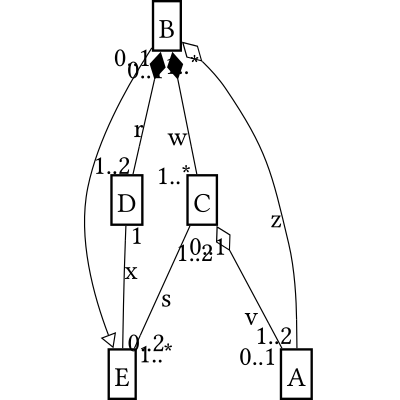
\includegraphics[min width=0.4\textwidth=0.6\textwidth,min height=0.4\textwidth=0.6\textwidth,keepaspectratio,max width=0.9\textwidth,max height=0.9\textwidth]{52/cdd98fa5f9699f7f24fc7953cf62b89e3298c6ff397cc23315cb8f3389b466b03201af83b04c596701db35357ce8aed00a3a92e08161.pdf}\end{centering}



Now consider the following object diagram, which is an instance of this class diagram:



\begin{centering}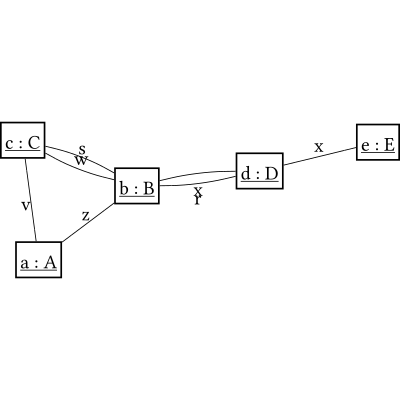
\includegraphics[min width=0.4\textwidth=0.6\textwidth,min height=0.4\textwidth=0.6\textwidth,keepaspectratio,max width=0.9\textwidth,max height=0.9\textwidth]{52/odb3dd8f1d0590ffb74d7617dd795cf3342662f4976d2517c3ac02a7745796030013.pdf}\end{centering}



